This section contains the main problem for this project and the form of solution required.
Further the scope and the limitations are also defined here.
\subsection{The problem}
The basis of this project is Aalborg Bycyklen, detailed in \cref{aalborg_bycyklen}.
The challenges described in \cref{aalborg_bycyklen:challenges} are the ones that needs to be solved.
The main problems are to:
\begin{itemize}
\item Improve flexibility
\item Improve reliability
\item Find lost bikes
\item Handle repairment of bikes
\end{itemize}

\subsection{Solution}
The biggest change to the current system, will be the addition of GPSs in the bikes.
This will provide the following opportunities:
\begin{itemize}
\item It will be possible to track the position of bikes.
\item Bike stations will be completely obsolete, instead 'hot-spots' will be introduced.
\item It will be possible to monitor the usage of bikes, thus statistical predictions on future locations and behavior will be possible.
\end{itemize}

\paragraph{Bike stations are unnecessary}
So far, bike stations serve a limited purpose.
They are where people are supposed to place the bikes after use, thus making it possible for other people to find the bikes.
However, bikes are not necessarily returned to a station after use, somewhat disrupting the sole purpose of the bike stations.

\paragraph{GPS}
Furthermore, by adding GPSs to the bikes, it will be possible to get an exact location of a bike, even if it is not at a bike station.
By monitoring the location of the bikes, their movements could be tracked.
Further, by detecting long stops (meaning ended trip), so-called hot-spots could be determined.

\paragraph{Hot-spot}
A hot-spot is an area, like an informal station.
But hot-spots come and go, depending on the use of the bikes.
A hot-spot is initialized when several bikes are available at the hot-spot location.
This is determined by looking at the history of the bike usage.

\paragraph{Locating bikes}
By requesting GPS locations from the bikes, it will be possible to get an overview of all bikes.
The system may then select an available bike nearby and guide the user to its location.
It can also be used by Aalborg Kommune, to locate missing or stolen bikes.

In regards to users locating bikes, they should have a more limited view, as compared to Aalborg Kommune.
They should be restricted to viewing bikes that are available and nearby.
A bike will be deemed available if it has been inactive for a given period of time.

If a bike should leave the Aalborg area, Aalborg Kommune should be notified.
If a bike is inactive for too long, it could mean that it is broken or parked too far away for anyone to use it.
Then Aalborg Kommune could be notified, so someone can either repair or move it.

\paragraph{Structure of the solution}
The structure of the solution can be seen in \cref{fig:solution_structure}.
The figure illustrates the software systems running on a server and what each system interact with.

The location service continuously request GPS data from the bikes and stores it in the database.

The web service handles requests from the users and returns a result based on the data in the database.

The inactivity agent continuously look in the database to check if a bike has been inactive for too long, then notifies Aalborg Kommune.

\subsection{Limitations}
The limits presented in the list below:
\begin{itemize}
\item Time: The project is due the 19th December 2014.
\item There is not provided any money for the project.
\end{itemize}

\subsection{Scope}
Because of the limitations mentioned above this project will be developing a webservice, a location service and an agent.
Which can be seen on \cref{fig:solution_structure} in the blue box.
 \alexander{Not necessary to have multiple agents? \giovanni{agent system?}}
 
 \begin{figure}[H]
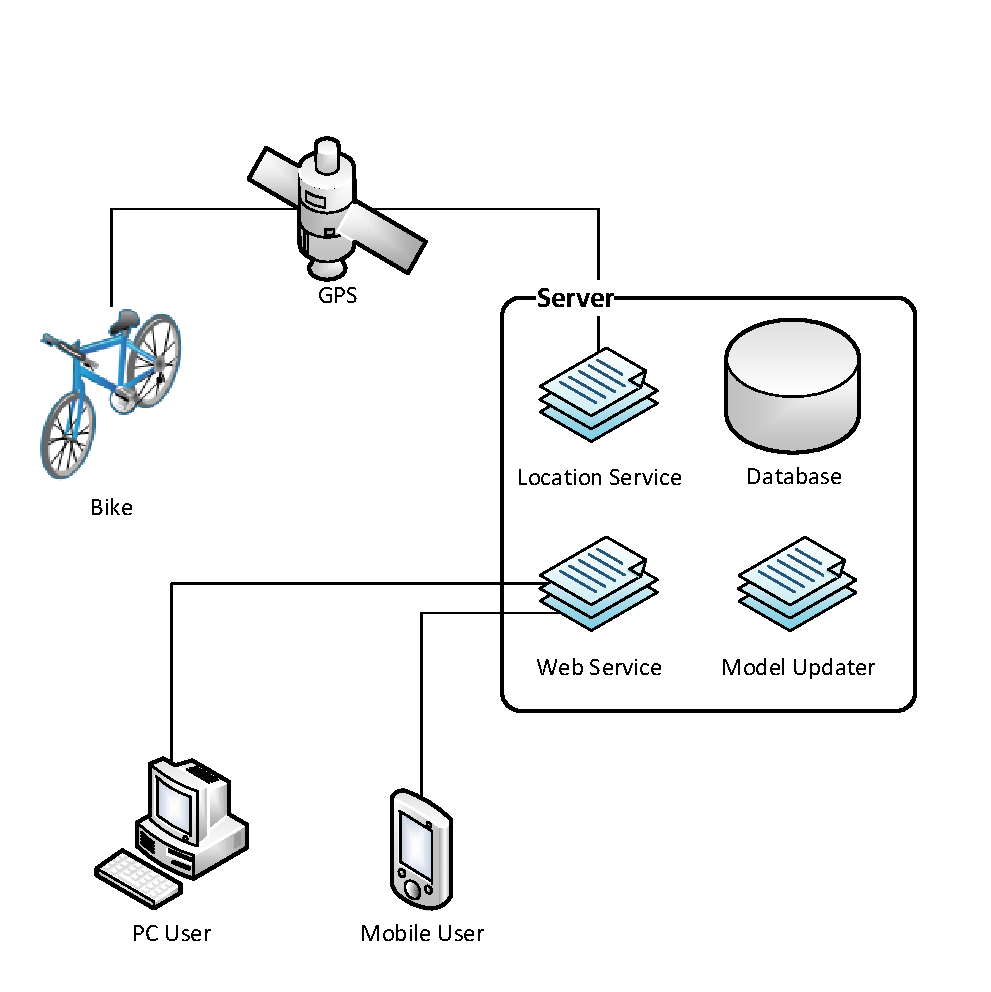
\includegraphics[width=\textwidth]{our_solution.pdf}
\caption{The overall structure of our solution}
\label{fig:solution_structure}
\end{figure}